%%%%%%%%%%%%%%%%%%%%%%%%%%%%%%%%%%%%%%%%%%%%%%%%%%%%%%%%%%%%%%%%%%%%%%%%%%%%%%%%%%%%
% Configuración de Paquetes
\documentclass{article}
\usepackage[framemethod=TikZ]{mdframed}
\usepackage{booktabs}
\usepackage{float}
\usepackage{scrextend}
\usepackage{titletoc}
\usepackage[margin=1in]{geometry} 
\usepackage{amsmath,amsthm,amssymb,amsfonts, fancyhdr, color, comment, graphicx, environ}
\usepackage{xcolor}
\usepackage{mdframed}
\usepackage[shortlabels]{enumitem}
\usepackage{indentfirst}
\usepackage{hyperref}
\usepackage{listings}
\usepackage{tikz}
\usepackage[framemethod=TikZ]{mdframed}
\usepackage{mathptmx}
\usepackage{cfr-lm}
\usepackage{color}
\hypersetup{
    colorlinks=true,
    linkcolor=blue,
    filecolor=magenta,      
    urlcolor=blue,
}
\setlength{\headheight}{1.5cm}
\renewcommand{\qed}{\quad\qedsymbol}
\usetikzlibrary{calc}
\renewcommand{\familydefault}{\sfdefault}
%%%%%%%%%%%%%%%%%%%%%%%%%%%%%%%%%%%%%%%%%%%%%%%%%%%%%%%%%%%%%%%%%%%%%%%%%%%%%%%%%%%%

\fancypagestyle{mipagina}{
    \fancyhf{} % Limpiar encabezado y pie de página
    \fancyhead[L]{Pedro Villar} % Nombre a la izquierda
    \fancyhead[C]{\rightmark} % Texto al centro 
    \fancyhead[R]{Org. del Computador} % Texto a la derecha
    \fancyfoot[C]{\thepage} % Número de página al centro
    \renewcommand{\headrulewidth}{0.4pt} % Grosor de la línea horizontal en el encabezado
}

\pagestyle{mipagina}
\mdfsetup{skipabove=\topskip,skipbelow=\topskip}

% Box de Definición
\newcounter{def}[section]

\NewDocumentEnvironment{defi}{o}{%
    \stepcounter{def}%
    \begin{mdframed}[
        frametitle={%
            \begin{tikzpicture}[baseline=(current bounding box.east),outer sep=0pt]
                \node[anchor=east,rectangle,fill=blue!20,inner xsep=5pt] at (0,0) {\strut\IfValueTF{#1}{Definición~\thedef:~#1}{Definición~\thedef}};
            \end{tikzpicture}%
        },
        innertopmargin=5pt,
        linecolor=blue!20,
        linewidth=2pt,
        topline=true,
        frametitleaboveskip=-\ht\strutbox, % Ajuste de espacio entre título y contenido
        frametitlealignment={\hspace{5pt}}, % Ajuste de espacio entre el borde del frame y el título
    ]
}{%
    \end{mdframed}%
}

% Box de ejemplos
\newcounter{ejemplo}[section]

\NewDocumentEnvironment{ejemplo}{o}{%
    \stepcounter{ejemplo}%
    \begin{mdframed}[
        frametitle={%
            \begin{tikzpicture}[baseline=(current bounding box.east),outer sep=0pt]
                \node[anchor=east,rectangle,fill=brown!30,inner xsep=5pt] at (0,0) {\strut\IfValueTF{#1}{Ejemplo~\theejemplo:~#1}{Ejemplo~\theejemplo}};
            \end{tikzpicture}%
        },
        innertopmargin=5pt,
        linecolor=brown!30,
        linewidth=2pt,
        topline=true,
        frametitleaboveskip=-\ht\strutbox, % Ajuste de espacio entre título y contenido
        frametitlealignment={\hspace{5pt}}, % Ajuste de espacio entre el borde del frame y el título
    ]
}{%
    \end{mdframed}%
}

% Entorno para Métodos (color verde)
\newcounter{metodo}[section]
\NewDocumentEnvironment{metodo}{o}{%
    \stepcounter{metodo}%
    \begin{mdframed}[
        frametitle={%
            \begin{tikzpicture}[baseline=(current bounding box.east),outer sep=0pt]
                \node[anchor=east,rectangle,fill=green!30,inner xsep=5pt] at (0,0) {\strut\IfValueTF{#1}{Método~\themetodo:~#1}{Método~\themetodo}};
            \end{tikzpicture}%
        },
        innertopmargin=5pt,
        linecolor=green!30,
        linewidth=2pt,
        topline=true,
        frametitleaboveskip=-\ht\strutbox, % Ajuste de espacio entre título y contenido
        frametitlealignment={\hspace{5pt}}, % Ajuste de espacio entre el borde del frame y el título
    ]
}{%
    \end{mdframed}%
}

% Entorno para Observaciones (color amarillo más oscuro)
\newcounter{observacion}[section]
\NewDocumentEnvironment{observacion}{o}{%
    \stepcounter{observacion}%
    \begin{mdframed}[
        frametitle={%
            \begin{tikzpicture}[baseline=(current bounding box.east),outer sep=0pt]
                \node[anchor=east,rectangle,fill=yellow!50,inner xsep=5pt] at (0,0) {\strut\IfValueTF{#1}{Observación~\theobservacion:~#1}{Observación~\theobservacion}};
            \end{tikzpicture}%
        },
        innertopmargin=5pt,
        linecolor=yellow!50,
        linewidth=2pt,
        topline=true,
        frametitleaboveskip=-\ht\strutbox, % Ajuste de espacio entre título y contenido
        frametitlealignment={\hspace{5pt}}, % Ajuste de espacio entre el borde del frame y el título
    ]
}{%
    \end{mdframed}%
}

% Entorno para Ejercicio
\newcounter{ejer}[section]
\NewDocumentEnvironment{ejer}{o}{%
    \stepcounter{ejer}%
    \begin{mdframed}[
        frametitle={%
            \begin{tikzpicture}[baseline=(current bounding box.east),outer sep=0pt]
                \node[anchor=east,rectangle,fill=black!30,inner xsep=5pt] at (0,0) {\strut\IfValueTF{#1}{Ejercicio~\theejer:~#1}{Ejercicio~\theejer}};
            \end{tikzpicture}%
        },
        innertopmargin=5pt,
        linecolor=black!30,
        linewidth=2pt,
        topline=true,
        frametitleaboveskip=-\ht\strutbox, % Ajuste de espacio entre título y contenido
        frametitlealignment={\hspace{5pt}}, % Ajuste de espacio entre el borde del frame y el título
    ]
}{%
    \end{mdframed}%
}

\newenvironment{solution}
    {\textit{Solución:}}
    {}

%Configuraciones adicionales
\binoppenalty=\maxdimen 
\relpenalty=\maxdimen 
\setlength{\parindent}{0pt}

\begin{document}

\section*{Ejercicio 1}
Convertir los siguientes números en hexadecimal a binario de $32$ bits:
\begin{enumerate}[a)]
    \item $0xABCDEF00$
    \item $0x123456$
    \item $0x8E3FC581$
    \item $0x10A6F2B$
\end{enumerate}

\begin{solution}
\textbf{Punto a)}
\begin{equation*}
    \underbrace{A}_{1010}\underbrace{B}_{1011}\underbrace{C}_{1100}\underbrace{D}_{1101}\underbrace{E}_{1110}\underbrace{F}_{1111}\underbrace{0}_{0000}\underbrace{0}_{0000}
\end{equation*}
\textbf{Punto b)}
\begin{equation*}
    \underbrace{1}_{0001}\underbrace{2}_{0010}\underbrace{3}_{0011}\underbrace{4}_{0100}\underbrace{5}_{0101}\underbrace{6}_{0110}
\end{equation*}
\textbf{Punto c)}
\begin{equation*}
    \underbrace{8}_{1000}\underbrace{E}_{1110}\underbrace{3}_{0011}\underbrace{F}_{1111}\underbrace{C}_{1100}\underbrace{5}_{0101}\underbrace{8}_{1000}\underbrace{1}_{0001}
\end{equation*}
\textbf{Punto d)}
\begin{equation*}
    \underbrace{1}_{0001}\underbrace{0}_{0000}\underbrace{A}_{1010}\underbrace{6}_{0110}\underbrace{F}_{1111}\underbrace{2}_{0010}\underbrace{B}_{1011}
\end{equation*}
\end{solution}

{\color{green} Ejercicio chequeado}

\section*{Ejercicio 2}
Convertir los siguientes números en binario a decimal y a hexadecimal:
\begin{enumerate}[a)]
    \item $(1110011110000011)_2$
    \item $(10110111001101000101111)_2$
    \item $(10110011011011.11000010000)_2$
    \item $(10001111110100011111.000001101)_2$
\end{enumerate}

El procedimiento va a ser el siguiente, primero tomo de derecha a izquierda en grupos de a $4$ bits, y asi convierto a hexadecimal. Luego, convierto a decimal.

\begin{solution}
\textbf{Punto a)}
\begin{equation*}
    \underbrace{1110}_{E}\underbrace{0111}_{7}\underbrace{1000}_{8}\underbrace{0011}_{3}
\end{equation*}
\begin{equation*}
    (1110011110000011)_2 = 0xE783 = 59267
\end{equation*}
\textbf{Punto b)}
En este caso no se puede agrupar de a $4$ bits sin que sobren bits, por lo que se agrega un $0$ a la izquierda:
\begin{equation*}
    \underbrace{0101}_{5}\underbrace{1011}_{B}\underbrace{1001}_{9}\underbrace{1010}_{A}\underbrace{0010}_{2}\underbrace{1111}_{F}
\end{equation*}
\begin{equation*}
    (10110111001101000101111)_2 = 0x5B9A2F = 6003247
\end{equation*}
\textbf{Punto c)}
Ahora se separa en dos partes, la parte entera y la parte fraccionaria, primero pongo la parte entera:
\begin{equation*}
    \underbrace{0010}_{2}\underbrace{1100}_{C}\underbrace{1101}_{D}\underbrace{1011}_{B}
\end{equation*}
\begin{equation*}
    \underbrace{1100}_{C}\underbrace{0010}_{2}\underbrace{0000}_{0}
\end{equation*}
\begin{equation*}
    (10110011011011.11000010000)_2 = 0x2CDB.C20 = 11483 + 12\cdot 16^{-1} + 2\cdot 16^{-2} = 11483.75
\end{equation*}
\textbf{Punto d)}
\begin{equation*}
    \underbrace{1000}_{8}\underbrace{1111}_{F}\underbrace{1011}_{D}\underbrace{0001}_{1}\underbrace{1111}_{F}
\end{equation*}
\begin{equation*}
    \underbrace{0000}_{0}\underbrace{0110}_{6}\underbrace{1000}_{8}
\end{equation*}
\begin{equation*}
    (10001111110100011111.000001101)_2 = 0x8FD1F.068 = 589087 + 0\cdot 16^{-1} + 6\cdot 16^{-2} + 8 \cdot 16^{-3} = 589087.033
\end{equation*}
\end{solution}

{\color{green} Ejercicio chequeado}

\section*{Ejercicio 3}
Suponiendo que se tienen registros de 16 bits, convertir a binario sin signo los siguientes números en base 10:
\begin{enumerate}[a)]
    \item $(123)_{10}$
    \item $(59)_{10}$
    \item $(255,46)_{10}$
    \item $(98,019)_{10}$
\end{enumerate}

\textbf{Punto a:} Para convertir a binario sin signo, se divide el número por $2$ y se toma el residuo, y se sigue dividiendo hasta que el cociente sea $0$. Luego se toman los residuos de abajo hacia arriba.

\begin{solution}
\textbf{Punto a)}
\begin{align*}
    123/2 &= 61 \quad \text{residuo } 1\\
    61/2 &= 30 \quad \text{residuo } 1\\
    30/2 &= 15 \quad \text{residuo } 0\\
    15/2 &= 7 \quad \text{residuo } 1\\
    7/2 &= 3 \quad \text{residuo } 1\\
    3/2 &= 1 \quad \text{residuo } 1\\
    1/2 &= 0 \quad \text{residuo } 1
\end{align*}

Por lo que el número en binario es $0000000001111011$.

\textbf{Punto b)}
\begin{align*}
    59/2 &= 29 \quad \text{residuo } 1\\
    29/2 &= 14 \quad \text{residuo } 1\\
    14/2 &= 7 \quad \text{residuo } 0\\
    7/2 &= 3 \quad \text{residuo } 1\\
    3/2 &= 1 \quad \text{residuo } 1\\
    1/2 &= 0 \quad \text{residuo } 1
\end{align*}

Por lo que el número en binario es $000000000111011$.

\newpage
\textbf{Punto c)}
Para convertir la parte entera, se sigue el mismo procedimiento que en los puntos anteriores. Para la parte fraccionaria, se multiplica por $2$ y se toma la parte entera, y se sigue multiplicando hasta que la parte fraccionaria sea $0$.

\begin{align*}
    255/2 &= 127 \quad \text{residuo } 1\\
    127/2 &= 63 \quad \text{residuo } 1\\
    63/2 &= 31 \quad \text{residuo } 1\\
    31/2 &= 15 \quad \text{residuo } 1\\
    15/2 &= 7 \quad \text{residuo } 1\\
    7/2 &= 3 \quad \text{residuo } 1\\
    3/2 &= 1 \quad \text{residuo } 1\\
    1/2 &= 0 \quad \text{residuo } 1
\end{align*}

Ahora para convertir la parte fraccionaria multiplicamos por $2$ y tomamos la parte entera:

\begin{align*}
    0.46 \cdot 2 &= 0.92 \quad \text{parte entera } 0\\
    0.92 \cdot 2 &= 1.84 \quad \text{parte entera } 1\\
    0.84 \cdot 2 &= 1.68 \quad \text{parte entera } 1\\
    0.68 \cdot 2 &= 1.36 \quad \text{parte entera } 1\\
    0.36 \cdot 2 &= 0.72 \quad \text{parte entera } 0\\
    0.72 \cdot 2 &= 1.44 \quad \text{parte entera } 1\\
    0.44 \cdot 2 &= 0.88 \quad \text{parte entera } 0\\
    0.88 \cdot 2 &= 1.76 \quad \text{parte entera } 1\\
\end{align*}

Por lo que el binario es $11111111.01110101$.

\textbf{Punto d)}
\begin{align*}
    98/2 &= 49 \quad \text{residuo } 0\\
    49/2 &= 24 \quad \text{residuo } 1\\
    24/2 &= 12 \quad \text{residuo } 0\\
    12/2 &= 6 \quad \text{residuo } 0\\
    6/2 &= 3 \quad \text{residuo } 0\\
    3/2 &= 1 \quad \text{residuo } 1\\
    1/2 &= 0 \quad \text{residuo } 1
\end{align*}

Ahora para convertir la parte fraccionaria multiplicamos por $2$ y tomamos la parte entera:

\begin{align*}
    0.019 \cdot 2 &= 0.038 \quad \text{parte entera } 0\\
    0.038 \cdot 2 &= 0.076 \quad \text{parte entera } 0\\
    0.076 \cdot 2 &= 0.152 \quad \text{parte entera } 0\\
    0.152 \cdot 2 &= 0.304 \quad \text{parte entera } 0\\
    0.304 \cdot 2 &= 0.608 \quad \text{parte entera } 0\\
    0.608 \cdot 2 &= 1.216 \quad \text{parte entera } 1\\
    0.216 \cdot 2 &= 0.432 \quad \text{parte entera } 0\\
    0.432 \cdot 2 &= 0.864 \quad \text{parte entera } 0\\
    0.864 \cdot 2 &= 1.728 \quad \text{parte entera } 1\\
\end{align*}

Por lo que el binario es $1100010.000001001$.

\end{solution}

{\color{green} Ejercicio chequeado}

\section*{Ejercicio 4}
Suponiendo que un microprocesador utiliza registros de 8 bits y representación de números negativos en complemento a 2, muestre el contenido de estos registros al codificar en binario los siguientes números con signo:
\begin{enumerate}[a)]
    \item $-76_{10}$
    \item $-43_{10}$
    \item $+64_{10}$
    \item $-121_{10}$
\end{enumerate}

\begin{solution}
\textbf{Punto a)}
Primero paso a binario el número $76$:

\begin{align*}
    76/2 &= 38 \quad \text{residuo } 0\\
    38/2 &= 19 \quad \text{residuo } 0\\
    19/2 &= 9 \quad \text{residuo } 1\\
    9/2 &= 4 \quad \text{residuo } 1\\
    4/2 &= 2 \quad \text{residuo } 0\\
    2/2 &= 1 \quad \text{residuo } 0\\
    1/2 &= 0 \quad \text{residuo } 1
\end{align*}

Por lo que el número en binario es $01001100$. Ahora para convertir a complemento a $2$, se toma el complemento a $1$ y se suma $1$:

\begin{align*}
    01001100 &\rightarrow 10110011 + 1 = 10110100
\end{align*}

\textbf{Punto b)}
Primero paso a binario el número $43$:

\begin{align*}
    43/2 &= 21 \quad \text{residuo } 1\\
    21/2 &= 10 \quad \text{residuo } 1\\
    10/2 &= 5 \quad \text{residuo } 0\\
    5/2 &= 2 \quad \text{residuo } 1\\
    2/2 &= 1 \quad \text{residuo } 0\\
    1/2 &= 0 \quad \text{residuo } 1
\end{align*}

Por lo que el número en binario es $00101011$. Ahora para convertir a complemento a $2$, se toma el complemento a $1$ y se suma $1$:

\begin{align*}
    00101011 &\rightarrow 11010100 + 1 = 11010101
\end{align*}

\textbf{Punto c)}
Primero paso a binario el número $64$:

\begin{align*}
    64/2 &= 32 \quad \text{residuo } 0\\
    32/2 &= 16 \quad \text{residuo } 0\\
    16/2 &= 8 \quad \text{residuo } 0\\
    8/2 &= 4 \quad \text{residuo } 0\\
    4/2 &= 2 \quad \text{residuo } 0\\
    2/2 &= 1 \quad \text{residuo } 0\\
    1/2 &= 0 \quad \text{residuo } 1
\end{align*}

Por lo que el número en binario es $01000000$. Como es positivo, el complemento a $2$ es el mismo número.

\textbf{Punto d)}

Primero paso a binario el número $121$:

\begin{align*}
    121/2 &= 60 \quad \text{residuo } 1\\
    60/2 &= 30 \quad \text{residuo } 0\\
    30/2 &= 15 \quad \text{residuo } 0\\
    15/2 &= 7 \quad \text{residuo } 1\\
    7/2 &= 3 \quad \text{residuo } 1\\
    3/2 &= 1 \quad \text{residuo } 1\\
    1/2 &= 0 \quad \text{residuo } 1
\end{align*}

Por lo que el número en binario es $01111001$. Ahora para convertir a complemento a $2$, se toma el complemento a $1$ y se suma $1$:

\begin{align*}
    01111001 &\rightarrow 10000110 + 1 = 10000111
\end{align*}
\end{solution}

{\color{green} Ejercicio chequeado}

\section*{Ejercicio 5}
Convertir los siguientes valores binarios de 8 bits en formato de complemento a dos a decimal:

\begin{enumerate}[a)]
    \item $10010110$
    \item $11111011$
    \item $11100000$
    \item $00011110$
\end{enumerate}

\begin{solution}
\textbf{Punto a)}
El número es negativo, por lo que se toma el complemento a $2$ y se suma $1$:

\begin{align*}
    10010110 &\rightarrow 01101001 + 1 = 01101010
\end{align*}

Por lo que el número en decimal es $-106$.

\textbf{Punto b)}
El número es negativo, por lo que se toma el complemento a $2$ y se suma $1$:

\begin{align*}
    11111011 &\rightarrow 00000100 + 1 = 00000101
\end{align*}

Por lo que el número en decimal es $-5$.

\textbf{Punto c)}
El número es negativo, por lo que se toma el complemento a $2$ y se suma $1$:

\begin{align*}
    11100000 &\rightarrow 00011111 + 1 = 00100000
\end{align*}

Por lo que el número en decimal es $-32$.

\textbf{Punto d)}
El número es positivo, por lo que el número en decimal es $30$.

\end{solution}

{\color{green} Ejercicio chequeado}

\section*{Ejercicio 6}
Suponga que los registros $A$ y $B$ del microprocesador del ejercicio $4$ (registros de 8 bits) contienen los valores $0x80$ y $0xD0$ respectivamente.
\begin{enumerate}[a)]
    \item ¿Qué valor contiene el registro C después de ejecutar la operación C = A + B?
    \newline ¿El resultado que se guarda en C es el esperado?
    \item ¿Qué valor contiene el registro C después de ejecutar la operación C = A - B?
    \newline ¿El resultado que se guarda en C es el esperado?
    \item En base al análisis de las operaciones anteriores, ¿cuál es la ventaja de la
    representación de números negativos mediante su complemento a 2, por sobre la
    representación binaria regular + un bit de signo?
\end{enumerate}

\begin{solution}
\textbf{Punto a)}
Primero paso a binario los números $0x80$ y $0xD0$:

\begin{align*}
    0x80 &= 10000000\\
    0xD0 &= 11010000
\end{align*}

Ahora sumo los números:

\begin{align*}
    10000000 + 11010000 &= 101010000
\end{align*}

El resultado es $0xA0$, por lo que el resultado no es el esperado.

\textbf{Punto b)}

Ahora resto utilizando complemento a $2$:

\begin{align*}
    10000000 - 11010000 &= 10000000 + 00110000 = 10110000
\end{align*}

El resultado es $0xB0$, por lo que el resultado no es el esperado.

\textbf{Punto c)}

La ventaja de la representación de números negativos mediante su complemento a $2$ es que se pueden realizar operaciones aritméticas sin tener que preocuparse por el signo, ya que el complemento a $2$ se encarga de que las operaciones aritméticas se realicen de la misma manera que con números positivos.

\end{solution}

{\color{green} Ejercicio chequeado}

\newpage

\section*{Ejercicio 7}
Expresar los siguientes números decimales en su representación binaria (negativos en complemento a 2) considerando los tamaños de los registros donde serán alojados según la tabla.

\begin{figure}[h]
    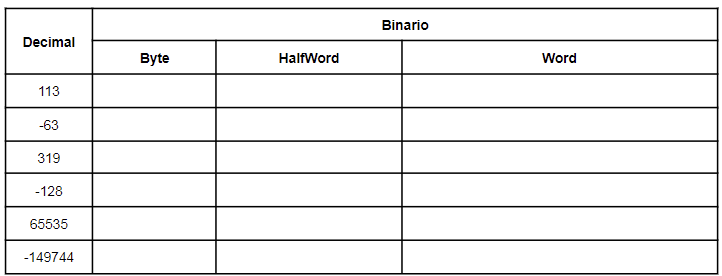
\includegraphics[width=1\textwidth]{tabla.png}
\end{figure}

\subsection*{Conceptos}
\begin{itemize}
    \item \textbf{Byte:} Un byte es una secuencia de $8$ bits.
    \item \textbf{HalfWord:} Un halfword es una secuencia de $16$ bits.
    \item \textbf{Word:} Un word es una secuencia de $32$ bits.
\end{itemize}

\begin{solution}
\textbf{Número 113}
Primero lo paso a binario:

\begin{align*}
    113/2 &= 56 \quad \text{residuo } 1\\
    56/2 &= 28 \quad \text{residuo } 0\\
    28/2 &= 14 \quad \text{residuo } 0\\
    14/2 &= 7 \quad \text{residuo } 0\\
    7/2 &= 3 \quad \text{residuo } 1\\
    3/2 &= 1 \quad \text{residuo } 1\\
    1/2 &= 0 \quad \text{residuo } 1
\end{align*}

Por lo que el número en binario es $01110001$. Ahora lo paso a los formatos de la tabla:

\begin{itemize}
    \item \textbf{Byte:} $01110001$
    \item \textbf{HalfWord:} $0000000001110001$
    \item \textbf{Word:} $00000000000000000000000001110001$
\end{itemize}

\textbf{Número -63}
Primero paso a binario el número $63$:

\begin{align*}
    63/2 &= 31 \quad \text{residuo } 1\\
    31/2 &= 15 \quad \text{residuo } 1\\
    15/2 &= 7 \quad \text{residuo } 1\\
    7/2 &= 3 \quad \text{residuo } 1\\
    3/2 &= 1 \quad \text{residuo } 1\\
    1/2 &= 0 \quad \text{residuo } 1
\end{align*}

Ahora le hago el complemento a $2$:

\begin{align*}
    00111111 &\rightarrow 11000000 + 1 = 11000001
\end{align*}

Por lo que el número en binario es $11000001$. Ahora lo paso a los formatos de la tabla:

\begin{itemize}
    \item \textbf{Byte:} $11000001$
    \item \textbf{HalfWord:} $1111111111000001$
    \item \textbf{Word:} $11111111111111111111111111000001$
\end{itemize}

\textbf{Número 319}
Primero paso a binario el número $319$:

\begin{align*}
    319/2 &= 159 \quad \text{residuo } 1\\
    159/2 &= 79 \quad \text{residuo } 1\\
    79/2 &= 39 \quad \text{residuo } 1\\
    39/2 &= 19 \quad \text{residuo } 1\\
    19/2 &= 9 \quad \text{residuo } 1\\
    9/2 &= 4 \quad \text{residuo } 0\\
    4/2 &= 2 \quad \text{residuo } 0\\
    2/2 &= 1 \quad \text{residuo } 0\\
    1/2 &= 0 \quad \text{residuo } 1
\end{align*}

Por lo que el número en binario es $100011111$. Ahora lo paso a los formatos de la tabla:

\begin{itemize}
    \item \textbf{Byte:} No es posible representarlo como byte.
    \item \textbf{HalfWord:} $0000000010001111$
    \item \textbf{Word:} $00000000000000000000000100011111$
\end{itemize}

\textbf{Número -128}
Primero paso a binario el número $128$:

\begin{align*}
    128/2 &= 64 \quad \text{residuo } 0\\
    64/2 &= 32 \quad \text{residuo } 0\\
    32/2 &= 16 \quad \text{residuo } 0\\
    16/2 &= 8 \quad \text{residuo } 0\\
    8/2 &= 4 \quad \text{residuo } 0\\
    4/2 &= 2 \quad \text{residuo } 0\\
    2/2 &= 1 \quad \text{residuo } 0\\
    1/2 &= 0 \quad \text{residuo } 1
\end{align*}

Ahora le hago el complemento a $2$:

\begin{align*}
    10000000 &\rightarrow 01111111 + 1 = 10000000
\end{align*}

Por lo que el número en binario es $10000000$. Ahora lo paso a los formatos de la tabla:

\begin{itemize}
    \item \textbf{Byte:} $10000000$
    \item \textbf{HalfWord:} $1111111110000000$
    \item \textbf{Word:} $11111111111111111111111110000000$
\end{itemize}

\textbf{Número 65535}
Primero paso a binario el número $65535$:

\begin{align*}
    65535/2 &= 32767 \quad \text{residuo } 1\\
    32767/2 &= 16383 \quad \text{residuo } 1\\
    16383/2 &= 8191 \quad \text{residuo } 1\\
    8191/2 &= 4095 \quad \text{residuo } 1\\
    4095/2 &= 2047 \quad \text{residuo } 1\\
    2047/2 &= 1023 \quad \text{residuo } 1\\
    1023/2 &= 511 \quad \text{residuo } 1\\
    511/2 &= 255 \quad \text{residuo } 1\\
    255/2 &= 127 \quad \text{residuo } 1\\
    127/2 &= 63 \quad \text{residuo } 1\\
    63/2 &= 31 \quad \text{residuo } 1\\
    31/2 &= 15 \quad \text{residuo } 1\\
    15/2 &= 7 \quad \text{residuo } 1\\
    7/2 &= 3 \quad \text{residuo } 1\\
    3/2 &= 1 \quad \text{residuo } 1\\
    1/2 &= 0 \quad \text{residuo } 1
\end{align*}

Por lo que el número en binario es $1111111111111111$. Ahora lo paso a los formatos de la tabla:

\begin{itemize}
    \item \textbf{Byte:} No es posible representarlo como byte.
    \item \textbf{HalfWord:} $000000001111111111111111$
    \item \textbf{Word:} $0000000000000000000000001111111111111111$
\end{itemize}

\textbf{Número -149744}
Primero paso a binario el número $149744$:

\begin{align*}
    149744/2 &= 74872 \quad \text{residuo } 0\\
    74872/2 &= 37436 \quad \text{residuo } 0\\
    37436/2 &= 18718 \quad \text{residuo } 0\\
    18718/2 &= 9359 \quad \text{residuo } 0\\
    9359/2 &= 4679 \quad \text{residuo } 1\\
    4679/2 &= 2339 \quad \text{residuo } 1\\
    2339/2 &= 1169 \quad \text{residuo } 1\\
    1169/2 &= 584 \quad \text{residuo } 0\\
    584/2 &= 292 \quad \text{residuo } 0\\
    292/2 &= 146 \quad \text{residuo } 0\\
    146/2 &= 73 \quad \text{residuo } 0\\
    73/2 &= 36 \quad \text{residuo } 1\\
    36/2 &= 18 \quad \text{residuo } 0\\
    18/2 &= 9 \quad \text{residuo } 0\\
    9/2 &= 4 \quad \text{residuo } 1\\
    4/2 &= 2 \quad \text{residuo } 0\\
    2/2 &= 1 \quad \text{residuo } 0\\
    1/2 &= 0 \quad \text{residuo } 1
\end{align*}

Ahora le hago el complemento a $2$:

\begin{align*}
    100100100110110000 &\rightarrow 011011011001010000 + 1 = 011011011001010001
\end{align*}

Por lo que el número en binario es $011011011001010001$. Ahora lo paso a los formatos de la tabla:

\begin{itemize}
    \item \textbf{Byte:} No se puede representar.
    \item \textbf{HalfWord:} $0011001101100101$
    \item \textbf{Word:} $0000000000000000000000000110110110010101$
\end{itemize}

\end{solution}

{\color{green} Ejercicio chequeado}

\section*{Ejercicio 8}
Convertir los siguientes números decimales a formato IEEE 754 de precisión simple (normalizados):

\begin{enumerate}[a)]
    \item $5678_{10}$
    \item $306,59375_{10}$
    \item $723,125_{10}$
    \item $18,1953125_{10}$
    \item $-3020,993_{10}$
    \item $-0,000892$
\end{enumerate}
\newpage
\begin{solution}
\textbf{Punto a)}
\begin{enumerate}
    \item El bit de signo es $0$, ya que el número es positivo.
    \item Paso a binario el número $5678$:
    \begin{align*}
        5678/2 &= 2839 \quad \text{residuo } 0\\
        2839/2 &= 1419 \quad \text{residuo } 1\\
        1419/2 &= 709 \quad \text{residuo } 1\\
        709/2 &= 354 \quad \text{residuo } 1\\
        354/2 &= 177 \quad \text{residuo } 0\\
        177/2 &= 88 \quad \text{residuo } 1\\
        88/2 &= 44 \quad \text{residuo } 0\\
        44/2 &= 22 \quad \text{residuo } 0\\
        22/2 &= 11 \quad \text{residuo } 0\\
        11/2 &= 5 \quad \text{residuo } 1\\
        5/2 &= 2 \quad \text{residuo } 1\\
        2/2 &= 1 \quad \text{residuo } 0\\
        1/2 &= 0 \quad \text{residuo } 1
    \end{align*}
    Por lo que el número en binario es $1011000101110$. 
    \item Para normalizar muevo la coma tantos lugares como sea necesario para que quede un uno seguido por la parte fracccionaria:
    \begin{itemize}
        \item \textbf{Sin normalizar:} $1011000101110 \times 2^0$
        \item \textbf{Normalizado:} $1.011000101110 \times 2^{12}$
    \end{itemize}
    \item El exponente es $12$, por lo que el sesgo es $127$, por lo que el exponente es $139$ en binario, que es $10001011$.
    \item Para la parte fraccionaria, tomo los $23$ bits que siguen al punto, que son $01100010111000000000000$.
    \item Ahora conformo el numero con el bit de signo, el exponente y la parte fraccionaria:
    \begin{equation*}
        0 \ 10001011 \ 01100010111000000000000
    \end{equation*}
\end{enumerate}

\textbf{Punto b)}
\begin{enumerate}
    \item El bit de signo es $0$, ya que el número es positivo.
    \item Convierto la parte entera y la parte fraccionaria en binario:
    \begin{itemize}
        \item Parte entera:
        \begin{align*}
            306/2 &= 153 \quad \text{residuo } 0\\
            153/2 &= 76 \quad \text{residuo } 1\\
            76/2 &= 38 \quad \text{residuo } 0\\
            38/2 &= 19 \quad \text{residuo } 0\\
            19/2 &= 9 \quad \text{residuo } 1\\
            9/2 &= 4 \quad \text{residuo } 1\\
            4/2 &= 2 \quad \text{residuo } 0\\
            2/2 &= 1 \quad \text{residuo } 0\\
            1/2 &= 0 \quad \text{residuo } 1
        \end{align*}
        Por lo que la parte entera en binario es $100110010$.
        \item Parte fraccionaria:
        \begin{align*}
            0.59375 \cdot 2 &= 1.1875 \quad \text{parte entera } 1\\
            0.1875 \cdot 2 &= 0.375 \quad \text{parte entera } 0\\
            0.375 \cdot 2 &= 0.75 \quad \text{parte entera } 0\\
            0.75 \cdot 2 &= 1.5 \quad \text{parte entera } 1\\
            0.5 \cdot 2 &= 1 \quad \text{parte entera } 1
        \end{align*}
        Por lo que la parte fraccionaria en binario es $10011$.
    \end{itemize}
    \item Para normalizar muevo la coma tantos lugares como sea necesario para que quede un uno seguido por la parte fracccionaria:
        \begin{itemize}
            \item \textbf{Sin normalizar:} $100110010.10011 \times 2^8$
            \item \textbf{Normalizado:} $1.0011001010011 \times 2^{8}$
        \end{itemize}
    \item El exponente es $8$, por lo que el sesgo es $127$, por lo que el exponente es $135$ en binario, que es $100110010$.
    \item Para la parte fraccionaria, tomo los $23$ bits que siguen al punto, que son $00110010100110000000000$.
    \item Ahora conformo el numero con el bit de signo, el exponente y la parte fraccionaria:
    \begin{equation*}
        0 \ 100110010 \ 00110010100110000000000
    \end{equation*}
\end{enumerate}

\textbf{Punto c)}
\begin{enumerate}
    \item El bit de signo es $0$, ya que el número es positivo.
    \item Convierto la parte entera y la parte fraccionaria en binario:
    \begin{itemize}
        \item Parte entera:
        \begin{align*}
            723/2 &= 361 \quad \text{residuo } 1\\
            361/2 &= 180 \quad \text{residuo } 0\\
            180/2 &= 90 \quad \text{residuo } 0\\
            90/2 &= 45 \quad \text{residuo } 0\\
            45/2 &= 22 \quad \text{residuo } 1\\
            22/2 &= 11 \quad \text{residuo } 0\\
            11/2 &= 5 \quad \text{residuo } 1\\
            5/2 &= 2 \quad \text{residuo } 1\\
            2/2 &= 1 \quad \text{residuo } 0\\
            1/2 &= 0 \quad \text{residuo } 1
        \end{align*}
        Por lo que la parte entera en binario es $1011010011$.
        \item Parte fraccionaria:
        \begin{align*}
            0.125 \cdot 2 &= 0.25 \quad \text{parte entera } 0\\
            0.25 \cdot 2 &= 0.5 \quad \text{parte entera } 0\\
            0.5 \cdot 2 &= 1 \quad \text{parte entera } 1
        \end{align*}
        Por lo que la parte fraccionaria en binario es $001$.
    \end{itemize}
    \item Para normalizar muevo la coma tantos lugares como sea necesario para que quede un uno seguido por la parte fracccionaria:
        \begin{itemize}
            \item \textbf{Sin normalizar:} $1011010011.001 \times 2^9$
            \item \textbf{Normalizado:} $1.011010011001 \times 2^{10}$
        \end{itemize}
    \item El exponente es $19$, por lo que el sesgo es $127$, por lo que el exponente es $136$ en binario, que es $10001000$.
    \item Para la parte fraccionaria, tomo los $23$ bits que siguen al punto, que son $01101001100100000000000$.
    \item Ahora conformo el numero con el bit de signo, el exponente y la parte fraccionaria:
    \begin{equation*}
        0 \ 10001000 \ 01101001100100000000000
    \end{equation*}
\end{enumerate}

\textbf{Punto d)}
\begin{enumerate}
    \item El bit de signo es $0$, ya que el número es positivo.
    \item Convierto la parte entera y la parte fraccionaria en binario:
    \begin{itemize}
        \item Parte entera:
        \begin{align*}
            18/2 &= 9 \quad \text{residuo } 0\\
            9/2 &= 4 \quad \text{residuo } 1\\
            4/2 &= 2 \quad \text{residuo } 0\\
            2/2 &= 1 \quad \text{residuo } 0\\
            1/2 &= 0 \quad \text{residuo } 1
        \end{align*}
        Por lo que la parte entera en binario es $10010$.
        \item Parte fraccionaria:
        \begin{align*}
            0.1953125 \cdot 2 &= 0.390625 \quad \text{parte entera } 0\\
            0.390625 \cdot 2 &= 0.78125 \quad \text{parte entera } 0\\
            0.78125 \cdot 2 &= 1.5625 \quad \text{parte entera } 1\\
            0.5625 \cdot 2 &= 1.125 \quad \text{parte entera } 1\\
            0.125 \cdot 2 &= 0.25 \quad \text{parte entera } 0\\
            0.25 \cdot 2 &= 0.5 \quad \text{parte entera } 0\\
            0.5 \cdot 2 &= 1 \quad \text{parte entera } 1
        \end{align*}
        Por lo que la parte fraccionaria en binario es $0011001$.
    \end{itemize}
    \item Para normalizar muevo la coma tantos lugares como sea necesario para que quede un uno seguido por la parte fracccionaria:
        \begin{itemize}
            \item \textbf{Sin normalizar:} $10010.0011001 \times 2^4$
            \item \textbf{Normalizado:} $1.00100011001 \times 2^{100}$
        \end{itemize}
    \item El exponente es $4$, por lo que el sesgo es $127$, por lo que el exponente es $131$ en binario, que es $10000011$.
    \item Para la parte fraccionaria, tomo los $23$ bits que siguen al punto, que son $00100011001000000000000$.
    \item Ahora conformo el numero con el bit de signo, el exponente y la parte fraccionaria:
    \begin{equation*}
        0 \ 10000011 \ 00100011001000000000000
    \end{equation*}
\end{enumerate}

\textbf{Punto e)}
\begin{enumerate}
    \item El bit de signo es $1$, ya que el número es negativo.
    \item Convierto la parte entera y la parte fraccionaria en binario:
    \begin{itemize}
        \item Parte entera:
        \begin{align*}
            3020/2 &= 1510 \quad \text{residuo } 0\\
            1510/2 &= 755 \quad \text{residuo } 0\\
            755/2 &= 377 \quad \text{residuo } 1\\
            377/2 &= 188 \quad \text{residuo } 1\\
            188/2 &= 94 \quad \text{residuo } 0\\
            94/2 &= 47 \quad \text{residuo } 0\\
            47/2 &= 23 \quad \text{residuo } 1\\
            23/2 &= 11 \quad \text{residuo } 1\\
            11/2 &= 5 \quad \text{residuo } 1\\
            5/2 &= 2 \quad \text{residuo } 1\\
            2/2 &= 1 \quad \text{residuo } 0\\
            1/2 &= 0 \quad \text{residuo } 1
        \end{align*}
        Por lo que la parte entera en binario es $101111001100$.
        \item Parte fraccionaria:
        \begin{align*}
            0.993 \cdot 2 &= 1.986 \quad \text{parte entera } 1\\
            0.986 \cdot 2 &= 1.972 \quad \text{parte entera } 1\\
            0.972 \cdot 2 &= 1.944 \quad \text{parte entera } 1\\
            0.944 \cdot 2 &= 1.888 \quad \text{parte entera } 1\\
            0.888 \cdot 2 &= 1.776 \quad \text{parte entera } 1 \\
            0.776 \cdot 2 &= 1.552 \quad \text{parte entera } 1\\
            0.552 \cdot 2 &= 1.104 \quad \text{parte entera } 1\\
            0.104 \cdot 2 &= 0.208 \quad \text{parte entera } 0\\
            0.208 \cdot 2 &= 0.416 \quad \text{parte entera } 0\\
            0.416 \cdot 2 &= 0.832 \quad \text{parte entera } 0\\
            0.832 \cdot 2 &= 1.664 \quad \text{parte entera } 1\\
            0.664 \cdot 2 &= 1.328 \quad \text{parte entera } 1\\
        \end{align*}
        Por lo que la parte fraccionaria en binario es $111111100011$.
    \end{itemize}
    \item Para normalizar muevo la coma tantos lugares como sea necesario para que quede un uno seguido por la parte fracccionaria:
        \begin{itemize}
            \item \textbf{Sin normalizar:} $101111001100.111111100011 \times 2^{11}$
            \item \textbf{Normalizado:} $1.01111001100111111100011 \times 2^{11}$
        \end{itemize}
    \item El exponente es $11$, por lo que el sesgo es $127$, por lo que el exponente es $138$ en binario, que es $10001010$.
    \item Para la parte fraccionaria, tomo los $23$ bits que siguen al punto, que son $01111011100111111000110$.
    \item Ahora conformo el numero con el bit de signo, el exponente y la parte fraccionaria:
    \begin{equation*}
        1 \ 10001010 \ 01111001100111111100011
    \end{equation*}
\end{enumerate}

\textbf{Punto f)}
\begin{enumerate}
    \item El bit de signo es $1$, ya que el número es negativo.
    \item La parte entera es $0$, por lo que el exponente es $0$.
    \item Convierto la parte fraccionaria en binario:
    \begin{align*}
        0.000892 \cdot 2 &= 0.001784 \quad \text{parte entera } 0\\
        0.001784 \cdot 2 &= 0.003568 \quad \text{parte entera } 0\\
        0.003568 \cdot 2 &= 0.007136 \quad \text{parte entera } 0\\
        0.007136 \cdot 2 &= 0.014272 \quad \text{parte entera } 0\\
        0.014272 \cdot 2 &= 0.028544 \quad \text{parte entera } 0\\
        0.028544 \cdot 2 &= 0.057088 \quad \text{parte entera } 0\\
        0.057088 \cdot 2 &= 0.114176 \quad \text{parte entera } 0\\
        0.114176 \cdot 2 &= 0.228352 \quad \text{parte entera } 0\\
        0.228352 \cdot 2 &= 0.456704 \quad \text{parte entera } 0\\
        0.456704 \cdot 2 &= 0.913408 \quad \text{parte entera } 0\\
        0.913408 \cdot 2 &= 1.826816 \quad \text{parte entera } 1\\
        0.826816 \cdot 2 &= 1.653632 \quad \text{parte entera } 1\\
        0.653632 \cdot 2 &= 1.307264 \quad \text{parte entera } 1\\
        0.307264 \cdot 2 &= 0.614528 \quad \text{parte entera } 0\\
        0.614528 \cdot 2 &= 1.229056 \quad \text{parte entera } 1\\
        0.229056 \cdot 2 &= 0.458112 \quad \text{parte entera } 0\\
        0.458112 \cdot 2 &= 0.916224 \quad \text{parte entera } 0\\
        0.916224 \cdot 2 &= 1.832448 \quad \text{parte entera } 1\\
        0.832448 \cdot 2 &= 1.664896 \quad \text{parte entera } 1\\
        0.664896 \cdot 2 &= 1.329792 \quad \text{parte entera } 1\\
        0.329792 \cdot 2 &= 0.659584 \quad \text{parte entera } 0\\
        0.659584 \cdot 2 &= 1.319168 \quad \text{parte entera } 1\\
        0.319168 \cdot 2 &= 0.638336 \quad \text{parte entera } 0\\
        0.638336 \cdot 2 &= 1.276672 \quad \text{parte entera } 1\\
        0.276672 \cdot 2 &= 0.553344 \quad \text{parte entera } 0\\
        0.553344 \cdot 2 &= 1.106688 \quad \text{parte entera } 1\\
        0.106688 \cdot 2 &= 0.213376 \quad \text{parte entera } 0\\
        0.213376 \cdot 2 &= 0.426752 \quad \text{parte entera } 0\\
        0.426752 \cdot 2 &= 0.853504 \quad \text{parte entera } 0\\
        0.853504 \cdot 2 &= 1.707008 \quad \text{parte entera } 1\\
        0.707008 \cdot 2 &= 1.414016 \quad \text{parte entera } 1\\
        0.414016 \cdot 2 &= 0.828032 \quad \text{parte entera } 0\\
        0.828032 \cdot 2 &= 1.656064 \quad \text{parte entera } 1\\
    \end{align*}
    Por lo que la parte fraccionaria en binario es $000000000011010011101010100011011$.
    \item Para normalizar muevo la coma tantos lugares como sea necesario para que quede un uno seguido por la parte fracccionaria:
        \begin{itemize}
            \item \textbf{Sin normalizar:} $0.0000000000111010011101010100011011 \times 2^{-10}$
            \item \textbf{Normalizado:} $1.11010011101010100011011 \times 2^{-11}$
        \end{itemize}
    \item El exponente es $-11$, por lo que el sesgo es $127$, por lo que el exponente es $116$ en binario, que es $01110100$.
    \item Para la parte fraccionaria, tomo los $23$ bits que siguen al punto, que son $11010011101010100011011$.
    \item Ahora conformo el numero con el bit de signo, el exponente y la parte fraccionaria:
    \begin{equation*}
        1 \ 01110100 \ 11010011101010100011011
    \end{equation*}
    
\end{enumerate}
\end{solution}

{\color{green} Ejercicio chequeado}

\section*{Ejercicio 9}
Convertir los siguientes en formato IEEE 754 de precisión simple (normalizados) a números decimales:
\begin{enumerate}[a)]
    \item $1 1 0 0 0 1 0 1 1 0 0 0 0 0 0 0 0 0 0 0 0 1 1 0 0 0 0 0 0 0 0 0 b$
    \item $0 1 0 0 0 1 0 0 1 0 0 0 0 0 0 0 1 0 0 0 0 0 1 0 0 1 1 0 0 0 0 0 b$
    \item $0 1 0 0 0 0 1 0 0 1 0 1 0 0 0 0 0 0 0 0 0 0 0 0 0 0 0 0 0 0 0 0 b$
    \item $0 0 1 1 1 0 0 1 0 0 1 0 0 1 1 0 1 0 1 1 1 0 0 1 0 0 1 1 1 1 0 1 b$
    \item $1 0 1 1 1 0 1 0 1 0 1 1 0 1 1 0 0 0 1 1 0 0 0 0 1 0 1 0 1 0 0 1 b$
    \item $1 1 1 1 1 1 1 1 1 0 0 0 0 0 0 0 0 0 0 0 0 0 0 0 0 0 0 0 0 0 0 0 b$
\end{enumerate}

\begin{solution}
\textbf{Punto a)}
\begin{enumerate}
    \item El bit de signo es $1$, por lo que el número es negativo.
    \item El exponente es $10001011$, que en decimal es $139$, por lo que el sesgo es $127$, por lo que el exponente es $12$.
    \item La parte fraccionaria es $0 0 0 0 0 0 0 0 0 0 0 0 1 1 0 0 0 0 0 0 0 0 0$.
    \item La parte entera es $1$, por lo que el número es $-1.00000000000011000000000 \times 2^{12}$.
    \item Ahora lo desnormalizo: $-1000000000000.11 \times 2^{0}$.
    \item Para pasarlo a decimal hago la suma de las potencias de $2$:
    \begin{itemize}
        \item Parte entera: $2^{12}  =4096$
        \item Parte fraccionaria: $2^{-1} + 2^{-2} = 0.5 + 0.25 = 0.75$ 
    \end{itemize}
    \item Por lo que el número en decimal es $-4096.75_{10}$.
\end{enumerate}

\textbf{Punto b)}
\begin{enumerate}
    \item El bit de signo es $0$, por lo que el número es positivo.
    \item El exponente es $10001001$, que en decimal es $137$, por lo que el sesgo es $127$, por lo que el exponente es $10$.
    \item La parte fraccionaria es $00000001000001001100000$.
    \item La parte entera es $1$, por lo que el número es $1.00000001000001001100000 \times 2^{10}$
    \item Ahora lo desnormalizo: $10000000100.000100110 \times 2^{0}$.
    \item Para pasarlo a decimal hago la suma de las potencias de $2$:
    \begin{itemize}
        \item Parte entera: $2^2+2^10 = 4 + 1024 = 1028$ 
        \item Parte decimal: $2^{-4} + 2^{-7} + 2^{-8} = 0.07421875$
    \end{itemize}
    \item Por lo que el número en decimal es $1028.07421875_{10}$.
\end{enumerate}

\textbf{Punto c)}
\begin{enumerate}
    \item El bit de signo es $0$, por lo que el número es positivo.
    \item El exponente es $10000100$, que en decimal es $132$, por lo que el sesgo es $127$, por lo que el exponente es $5$.
    \item La parte fraccionaria es $10100000000000000000000$.
    \item La parte entera es $1$, por lo que el número es $1.10100000000000000000000 \times 2^{5}$
    \item Ahora lo desnormalizo: $110100.000000000000000000 \times 2^{0}$.
    \item Para pasarlo a decimal hago la suma de las potencias de $2$:
    \begin{itemize}
        \item Parte entera: $2^2+2^4+2^5 = 52$ 
    \end{itemize}
    \item Por lo que el número en decimal es $52_{10}$.
\end{enumerate}

\textbf{Punto d)}
\begin{enumerate}
    \item El bit de signo es $0$, por lo que el número es positivo.
    \item El exponente es $01110010$, que en decimal es $114$, por lo que el sesgo es $127$, por lo que el exponente es $-13$.
    \item La parte fraccionaria es $01001101011100100111101$.
    \item La parte entera es $1$, por lo que el número es $1.01001101011100100111101 \times 2^{-13}$
    \item Ahora lo desnormalizo: $0.00000000000011001101011100100111101 \times 2^{0}$.
    \item Para pasarlo a decimal hago la suma de las potencias de $2$:
    \begin{itemize}
        \item Parte entera: $0$ 
        \item Parte decimal: $0.00019592969329096$
    \end{itemize}
    \item Por lo que el número en decimal es $0.00019592969329096_{10}$.
\end{enumerate}

\textbf{Punto e)}
\begin{enumerate}
    \item El bit de signo es $1$, por lo que el número es negativo.
    \item El exponente es $01110101$, que en decimal es $117$, por lo que el sesgo es $127$, por lo que el exponente es $-10$.
    \item La parte fraccionaria es $01101100011000010101001$.
    \item La parte entera es $1$, por lo que el número es $-1.01101100011000010101001 \times 2^{-10}$
    \item Ahora lo desnormalizo: $-0.00000000011101100011000010101001 \times 2^{0}$.
    \item Para pasarlo a decimal hago la suma de las potencias de $2$:
    \begin{itemize}
        \item Parte entera: $0$ 
        \item Parte decimal: $0.001803437480703$
    \end{itemize}
    \item Por lo que el número en decimal es $-0.001803437480703_{10}$.
\end{enumerate}

\newpage
\textbf{Punto f)}
\begin{enumerate}
    \item El bit de signo es $1$, por lo que el número es negativo.
    \item El exponente es $11111111$, que en decimal es $255$, por lo que el sesgo es $127$, por lo que el exponente es $128$.
    \item La parte fraccionaria es $00000000000000000000000$.
    \item La parte entera es $1$, por lo que el número es $-1.00000000000000000000000 \times 2^{128}$
    \item Ahora lo desnormalizo: $-...00000000000000000000000 \times 2^{0}$.
    \textbf{El número es infinito negativo.}
\end{enumerate}
\end{solution}

{\color{green} Ejercicio chequeado}

\section*{Ejercicio 10}
Investigar cómo se escriben los símbolos especiales (“NaN”, “+Infinito”, “-Infinito”, “+0”, “-0”)
en formato IEEE 754 de precisión simple (normalizados).

\begin{solution}
    \begin{itemize}
        \item \textbf{NaN:} Para representar un NaN en formato IEEE 754 de precisión simple, se debe poner el bit de signo en $0$, el exponente en $11111111$ y la parte fraccionaria en cualquier valor distinto de $0$. Por ejemplo, $0 \ 11111111 \ 10000000000000000000000$.
        \item \textbf{+Infinito:} Para representar un $+\infty$ en formato IEEE 754 de precisión simple, se debe poner el bit de signo en $0$, el exponente en $11111111$ y la parte fraccionaria en $0$. Por ejemplo, $0 \ 11111111 \ 00000000000000000000000$.
        \item \textbf{-Infinito:} Para representar un $-\infty$ en formato IEEE 754 de precisión simple, se debe poner el bit de signo en $1$, el exponente en $11111111$ y la parte fraccionaria en $0$. Por ejemplo, $1 \ 11111111 \ 00000000000000000000000$.
        \item \textbf{+0:} Para representar un $+0$ en formato IEEE 754 de precisión simple, se debe poner el bit de signo en $0$, el exponente en $00000000$ y la parte fraccionaria en $0$. Por ejemplo, $0 \ 00000000 \ 00000000000000000000000$.
        \item \textbf{-0:} Para representar un $-0$ en formato IEEE 754 de precisión simple, se debe poner el bit de signo en $1$, el exponente en $00000000$ y la parte fraccionaria en $0$. Por ejemplo, $1 \ 00000000 \ 00000000000000000000000$.
    \end{itemize}
\end{solution}

{\color{green} Ejercicio chequeado}

\end{document}